\documentclass[a4paper, 12pt]{article}
\usepackage{comment} % enables the use of multi-line comments (\ifx \fi) 
\usepackage{lipsum} %This package just generates Lorem Ipsum filler text. 
\usepackage{fullpage} % changes the margin
\usepackage{hyperref}
\usepackage{graphicx}
\graphicspath{ {img/} }

\begin{document}
%Header-Make sure you update this information!!!!
\noindent
\begin{center}
\LARGE\textbf{CS 489 - P1 - Additive Synthesizer}\\
\large{Leah Dineen, Tyler Sanderson, Amanda Valoppi} \\
\large{Due Monday March 21, 2016 at 11:59 PM}


\end{center}

\section*{Introduction}
As described previously in the initial proposal, our culminating project is an additive synthesizer. Using synthesis techniques like LFO (low frequency oscillation), ADSR (attack, decay, sustain, release) envelopes, and linear convolution, users will be able to build unique sounds from the ground up with basic waveforms as their foundations. We also provide support for core audio effects, including delay and reverb. The final deliverable will be accessible via a web application, with a fully functional user interface, as well as basic keyboard support for note playback. In this progress report, we will outline implementation details of different aspects of our synthesizer, state planned additions for the final deliverable, and give an overview of the architecture of the project.

\section*{Project Access}
Currently, our project is available as a Github repository, at \url{https://github.com/leahdineen/audioProject}. To run it locally, simply clone the repository:
\begin{center}\emph{git clone https://github.com/leahdineen/audioProject.git}\end{center}

Finally, open the included \emph{index.html} in a browser. \textbf{NOTE: } Internet Explorer lacks support for the Web Audio API[1] (see \url{http://caniuse.com/#feat=audio-api}). Chrome or Firefox are preferred. There is currently support for playing one octave (12 semitones), starting at $A_4$, using the QWERTYIOP[] row of your keyboard.

\section*{Architecture Overview}
The sound processing pipeline for our synthesizer can be represented as a directed acyclic graph, containing nodes represented as audio effects, oscillators, waveform generators, and so forth. To get a better understanding, a diagram of the current pipeline is provided on the next page. Along with that, another diagram is included which outlines our final planned architecture.\\
 Currently, we start by generating one of a few basic waveforms (sine, square, triangle, sawtooth). The output is fed into a gain node, which regulates the volume. Then, we feed that into a pan node, which regulates the stereo pan. After the pan node, we feed the signal into an audio effects node, which applies effects like reverb and/or delay. Finally, we pipe our sound out to an output to be played back. It's important to note that LFOs and ADSR envelopes are optionally applied to the basic waveform, gain node, or pan node to oscillate and apply envelopes to chosen audio parameters.
 \newpage

\null
\vfill
\begin{center}
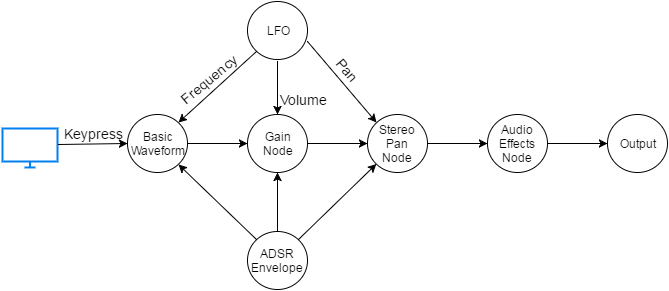
\includegraphics[scale=0.75]{architecture1.png}
Figure 1: Current audio processing pipeline
\end{center}
\vfill

\null
\vfill
\begin{center}
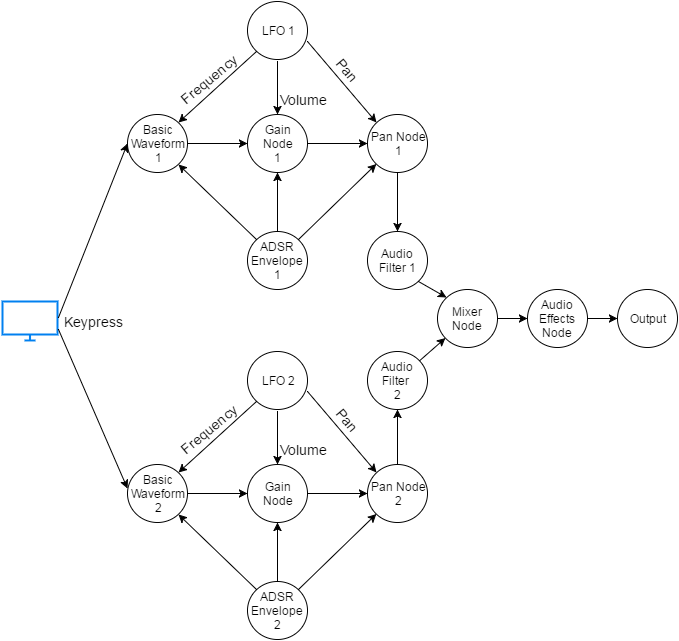
\includegraphics[scale=0.75]{architecture2.png}
Figure 2: Planned audio processing pipeline. Includes an additional waveform, mixer, and audio filters.
\end{center}
\vfill

\section*{Progress}

Currently, we have implemented many of our initially proposed features, along with functional user interface components. The audio processing pipeline in Figure 1 is currently how we handle sound generation for our synthesizer, while the pipeline in Figure 2 is what we hope to achieve for our final deliverable. In particular, here is a feature list outlining our progress and future steps:

\subsection*{Completed}
\begin{itemize}
\item Basic waveform generator for sine wave, square wave, triangle wave, and sawtooth wave
\item Polyphony to play arpeggios and chords
\item Phase shifting of basic waveforms
\item Volume control
\item Stereo pan control
\item ADSR envelope supporting volume, pan, and frequency envelopes
\item LFO supporting volume, pan, and frequency oscillation
\end{itemize}

\subsection*{In Progress for Final Deliverable}
\begin{itemize}
\item Second waveform generator
\item Second LFO
\item Second ADSR envelope
\item Mixer for separate waveform generators
\item Master audio effects (reverb, delay)
\item Audio filters (lowpass, highpass)
\end{itemize}
\section*{Implementation}

\subsection*{Basic Waveforms}

To generate our initial waveform to be used by an oscillator, we utilized a Web Audio API concept known as Wave Tables. A Wave Table is represented by two arrays of $N$ coefficients. One array contains all real parts (cosine coefficients) of the wave, while the other contains all imaginary parts (sine coefficients) of the wave. To construct the waveform, we simply build the appropriate Wave Table of Fourier Coefficients, and pass it into an OscillatorNode[2] to generate a periodic signal by summing up the components. Specifically, for each waveform, we set the imaginary Fourier Coefficients as follows (all real parts are zero since we are summing only the sine components):

\begin{itemize}
\item Sine
$$imag[1] = 1 \textnormal{ since we only need the fundamental frequency }$$
\item Square
$$imag[k] = \frac{4}{\pi k}, 1 \leq k \leq 4096, k \equiv 0 (mod 2)$$
\item Sawtooth
$$imag[k] = \frac{2(-1)^k}{\pi k}, 1 \leq k \leq 4096$$
\item Triangle
$$imag[k] = \frac{8(-1)^{\frac{k-1}{2}}}{\pi^2 k^2}, 1 \leq k \leq 4096, k \equiv 0 (mod 2)$$
\end{itemize}

This convenient for implementing a phase shift to our basic waveforms. To shift by $\phi$, we simply apply the following for each element in our arrays:

$$real[k] = real[k] * cos(2 \pi \phi) - imag[k] * sin(2 \pi \phi), \forall k$$
$$imag[k] = real[k] * sin(2 \pi \phi) - imag[k] * cos(2 \pi \phi), \forall k$$

\subsection*{ADSR Envelopes}

An ADSR (attack, decay, sustain, release) envelope is an abstraction for how the values of an audio parameter change over time. The attack time is how long the audio parameter takes to get to its peak value. The decay time is how long it takes to ramp down to its sustain level. Finally, the release time is how long on release the parameter takes to decay to zero. The schematic of an ADSR envelope is illustrated below:

\begin{center}
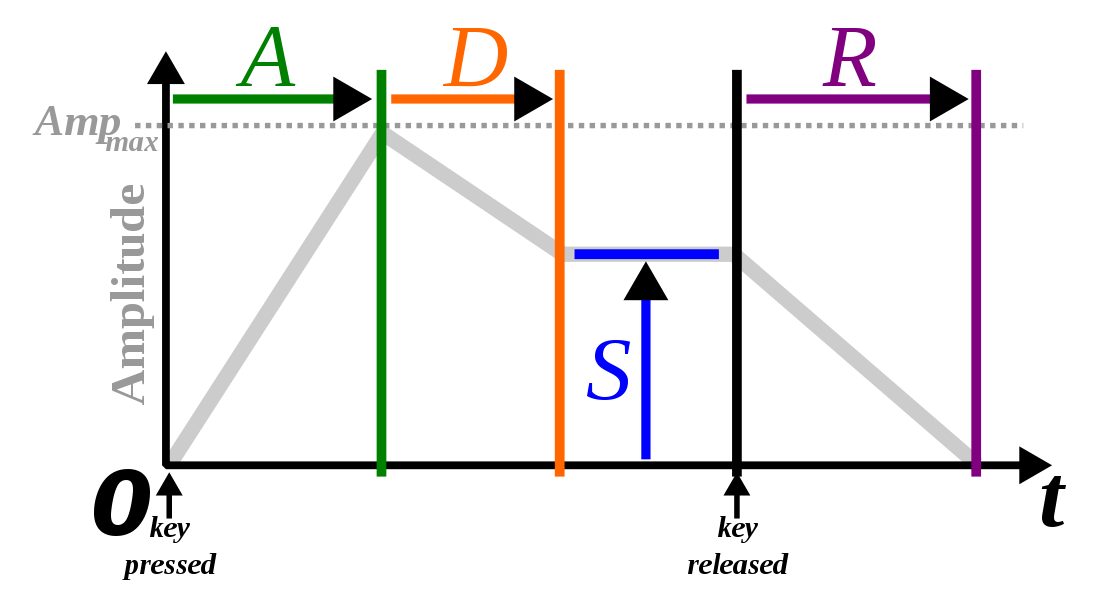
\includegraphics[scale=0.4]{adsr.png}
Figure 3: An ADSR envelope applied to amplitude
\end{center}

A key concept is that this envelope is an abstraction that can be applied to arbitrary audio parameters. On keypress, the value linearly increases to its peak based on the attack time. Then, it linearly decays down to its sustain level based on the decay time. On key release, the value linearly decreases down to zero based on its release time. The Web Audio API provides us with the handy interface AudioParam[3] that supports scheduling values, linearly ramping values, and more.

\subsection*{LFO}

A LFO (low-frequency oscillator) is simply an oscillator that generates a periodic waveform at a low frequency (usually below 20Hz), which can be used to modulate audio parameters. The frequency of the LFO waveform determines the rate of modulation (cycles per second), while the amplitude of the LFO waveform determines the intensity of modulation. It may be helpful to also think of an LFO as a function that takes a waveform as input, and operates on an audio paramter. The audio parameter changes its value based on the corresponding values of the waveform at sampling intervals. Consider this concrete example. We generate a sine wave with frequency 2Hz, and amplitude 1 with our LFO. Next, we connect our LFO to an audio parameter, say volume. Once we start the LFO, the value of the volume parameter will oscillate up and down by 1, 2 times a second, following the shape of the sine wave we generated.\\

In terms of implementation details, an LFO is essentially the same as our waveform generator, but with different amplitude and frequency values. As such, they can be implemented in the same way as detailed in the \emph{Basic Waveforms} above. It's important to note that different parameters should be modulated with different amplitude scales. For instance, if volume takes on the range $(0, 1)$, the amplitude range should be $(0, 1)$. However, for frequency, our range is much different, and is modulated based on semitones rather than raw values.

\subsection*{Pipeline}

We previously described our current audio processing pipeline as a directed acyclic graph. To implement this abstraction, we made use of the Web Audio API interface AudioNode[4], which provides essential tools to connect our pipeline properly. As mentioned before, a node can be an audio effect, an oscillator, or other arbitrary audio components. A node may also contain AudioParams[3] which can be modulated or regulated by ADSR envelopes. Using this information, to achieve polyphony, we can instantiate an individual instance of this audio pipeline for every note played, rather than only having one master pipeline to one master output.

\section*{Conclusion}

We currently have several key features completed for our additive synthesizer, and a much better understanding of the foundations of practical audio processing. Using concepts learned in lectures, along with the comprehensive Web Audio API for HTML 5, we have built a functioning version of a basic synthesizer. For our final deliverable, we plan to have most, if not all of the more advanced features detailed in the \emph{Progress} section completed.
\newpage

\section*{Notes}

\begin{enumerate}
\item Web Audio API\\
(source: \url{https://developer.mozilla.org/en-US/docs/Web/API/Web_Audio_API})

\item OscillatorNode - an abstraction for a waveform oscillator.\\
(source: \url{https://developer.mozilla.org/en-US/docs/Web/API/OscillatorNode})

\item AudioParam - an abstraction for a configurable audio parameter like volume, pan, or frequency.\\
(source: \url{https://developer.mozilla.org/en-US/docs/Web/API/AudioParam})

\item AudioNode - an abstraction for a node in our processing pipeline. Supports connecting to other nodes, and may contain individual audio parameters.\\
(source: \url{https://developer.mozilla.org/en-US/docs/Web/API/AudioNode})


\end{enumerate}

\section*{Resources}

\begin{itemize}

\item Reid, Gordon. "Synth Secrets." Sound on Sound. July 2004. Web. 9 Feb. 2016. \\
\url{http://www.soundonsound.com/sos/allsynthsecrets.htm} 

\item Smith, Julius O., III. Spectral Audio Signal Processing. Center for Computer Research in Music and Acoustics. Stanford University. Web. 9 Feb. 2016. \\
\url{https://ccrma.stanford.edu/~jos/sasp/}

\item "Synthesizer." Wikipedia. Web. 20 Mar. 2016.\\
\url{https://en.wikipedia.org/wiki/Synthesizer}

\item "Web Audio API." Mozilla. Web. 9 Feb. 2016. \\
\url{https://developer.mozilla.org/en-US/docs/Web/API/Web_Audio_API}


\end{itemize}

\end{document}
